
\documentclass[12pt]{standalone}
\usepackage{tikz}
\usetikzlibrary{calc, decorations.pathreplacing}

\begin{document}

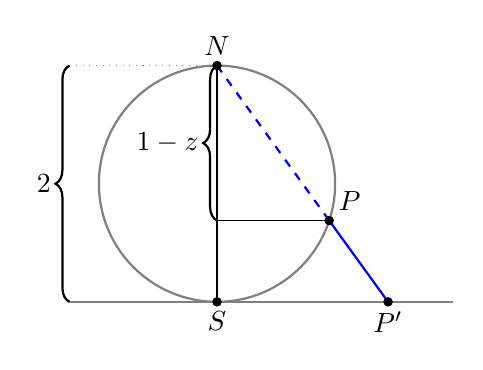
\begin{tikzpicture}[scale=1.5]
\coordinate (O) at (0,0);
\coordinate (N) at (0,1);
\coordinate (S) at (0,-1);
\coordinate (P) at (0.95, -0.3122);
\coordinate (P1) at (${2/(1+0.3122)}*(P)+{1-2/(1+0.3122)}*(N)$);
\draw[gray, thick] (O) circle(1);
\draw[gray, thick] (-1.25, -1) -- (2, -1);
\draw[gray, dotted] (-1.25, 1) -- (0, 1);
\draw (N) -- (S);
\draw (P) -- (P-|N);
\draw[decorate,decoration={brace,amplitude=5pt,mirror}, thick] 
(N) -- (P-|N) node[midway, left, xshift=-3pt] {$1-z$};
\draw[decorate,decoration={brace,amplitude=5pt,mirror}, thick] 
(-1.25,1) -- (-1.25,-1) node[midway, left, xshift=-3pt] {$2$};
\draw[dashed, blue, thick] (N) -- (P);
\draw[blue, thick] (P) -- (P1);
\filldraw (N) circle(1pt)  node[above] {$N$};
\filldraw (S) circle(1pt) node[below] {$S$};
\filldraw (P) circle(1pt) node[above right] {$P$};
\filldraw (P1) circle(1pt) node[below] {$P'$};
\end{tikzpicture}
\end{document}
